\documentclass{article}
%基于北京航空航天大学仪器科学与光电工程学院实验报告及课程报告排版得来,类似于毕业论文排版格式
%后续将更新毕业论文排版格式
\usepackage{graphicx,float}%使用图的宏包,使用图的浮动体宏包,引入参数H使图像紧跟当前文字
\usepackage{caption} %使用图表标题的宏包
\usepackage[colorlinks=true,pdfstartview=FitH,%
linkcolor=black,anchorcolor=violet,citecolor=magenta]{hyperref}%加载hyperref宏包,使用超链接
\usepackage{setspace}%用于设置行间距列间距等命令的宏包
\usepackage{array}%设置列表高度宽度的宏包
\usepackage{zhnumber}%使用中文数字编号的宏包
\usepackage{titlesec,titletoc}%使用标题自定义形式的宏包和使用目录自定义形式的宏包
\usepackage{siunitx}%物理学单位宏包
\usepackage{tabularx}%让表格宽度等于页面宽度
\usepackage{makecell}%单个表格单元调整的宏包
\usepackage{subfigure} %%使用子图的宏包
\usepackage{dirtree}
\usepackage[backend=biber,%nature,%%加载biblatex宏包,使用参考文献
gbnamefmt=quanpin,%将文献作者姓氏区分大小写
bibstyle=gb7714-2005,%加载参考文献样式表
maxbibnames=3,
%nature,%%加载biblatex宏包,使用参考文献
citestyle=gb7714-2005,%加载引注样式
%backref=false,%不显示引用文献的页码
gblocal=gb7714-2005,%使中英文献各自输入中英文的“和”与“等”
url=false,%注意,report类型文档类下,url和报告时间是必须的
doi=false,%不显示网址和doi
gbpunctin=false,%不显示文献中的//析出符号
gbmedium=false,%不显示OL符号
mergedate=none
]{biblatex}%标注(引用)样式citestyle,著录样式bibstyle都采用gb7714-2015样式
% \usepackage{pgfplots}%类似tikz的一个画图库,主要画统计图
\usepackage{../customStyle}
\addbibresource[location=local]{bibliography.bib}
\graphicspath{{./fig}}

\fancyhf{} 
% 页眉页脚设置
\lhead{公式推导部分}
\chead{陨石坑识别}
\rhead{\today}
\cfoot{\thepage}
\rfoot{}
\lfoot{}
% 加入页眉
\pagestyle{fancy}
% 表格行间距调整为1.5
% \renewcommand{\arraystretch}{1.5}

\begin{document}
\section{关于椭圆}
由于陨石坑的边缘始终是当作椭圆,因此在计算边缘、计算不确定度时大量使用到了椭圆的一般式和齐次矩阵,这里详细记录一遍。定义椭圆的一般式定义为:
\begin{equation}
  Ax^2+2Bxy+Cy^2+2Dx+2Ey+F=0\label{eq:ellipse}
\end{equation}\par
务必注意一般式定义中含有系数2,因此在椭圆的齐次矩阵中取消该系数:
\begin{equation}
  \mathbf{C}=\begin{bmatrix}
    A&B&D\\
    B&C&E\\
    D&E&F
  \end{bmatrix}
\end{equation}\par
\subsection{椭圆参数计算}
通过一般式求解椭圆的参数过程烦琐,但是可以算,解出椭圆的中心为:
\begin{equation*}
  \begin{cases}
    x_0=\frac{CD-BE}{B^2-AC}\\
    y_0=\frac{AE-BD}{B^2-AC}
  \end{cases}
\end{equation*}\par
椭圆的长短轴长度为:
\begin{equation*}
  \begin{cases}
    a^2=\frac{2(AE^2+CD^2+BF^2-2BDE-ACF)}{(B^2-AC)(\sqrt{(A-C)^2+4B^2}-A-C)}\\
    b^2=\frac{2(AE^2+CD^2+BF^2-2BDE-ACF)}{(B^2-AC)(-\sqrt{(A-C)^2+4B^2}-A-C)}
  \end{cases}\triangleq\begin{cases}
    a^2=\frac{2N_a}{D_a}\\
    b^2=\frac{2N_b}{D_b}
  \end{cases}
\end{equation*}\par
注意在求解过程中,经常因为椭圆被压扁为直线,导致解出来的$a^2$或$b^2$为负数,此时应当将这种情况舍去。
\subsection{不确定度}
计算椭圆的不确定度才是令人发指的,首先考察不确定度的由来,例如,对于同一个椭圆的边缘点,现有$n$个观测点$(x_i,y_i,1)$,则可利用奇异值分解算出椭圆一般式参数,如下式:
\begin{equation*}
  \begin{bmatrix}
    x_1^2&2x_1y_1&y^2_1&2x_1&2y_1&1\\
    x_2^2&2x_2y_2&y^2_2&2x_2&2y_2&1\\
    \vdots&\vdots&\vdots&\vdots&\vdots&\vdots\\
    x_n^2&2x_ny_n&y^2_n&2x_n&2y_n&1
\end{bmatrix}
  \begin{bmatrix}
    A\\B\\C\\D\\E\\F
  \end{bmatrix}=\mathbf{AX}=\mathbf{0}\implies\mathbf{U}\mathbold{\Sigma}\mathbf{ V}^\top=\mathbf{A}\implies\mathbf{X}=\mathbf{V}_6
\end{equation*}\par
即矩阵$\mathbf{V}$的最后一列是$\mathbf{X}$的解。此时求解不确定度,可将各个点的观测值当作对同一个椭圆的独立重复试验,且为了简化求解过程,将$\mathbf{X}$的六个分量当作服从相同噪声分布,且彼此独立,此时可根据最小二乘公式一步求出不确定度:
\begin{equation}
  \mathbf{D}=\frac{\mathbf{v^\top v}}{n-6}\mathbf{VV^\top}
  \label{eq:SVD}
\end{equation}\par
式中的$\mathbf{v=AX}$是正规方程的残差,虽然这样计算存在较多的简化和理想化结果,但是并不太影响最终的结果。接下来,可以从公式\ref{eq:SVD}中一步计算出六个参数的不确定度,即各自主对角线元素的算术平方根,如下式:
\begin{equation*}
  u(A)=\sqrt{D_{11}},u(B)=\sqrt{D_{22}},u(C)=\sqrt{D_{33}},u(D)=\sqrt{D_{44}},u(E)=\sqrt{D_{55}},u(F)=\sqrt{D_{66}}
\end{equation*}\par
利用本式,推导陨石坑中心点的不确定度,开根号即可:
\begin{equation}
  \begin{aligned}
    u^2(x_0)&=\left[\frac{CD-BE}{(B^2-AC)^2}\right]^2u^2(A)+\left[\frac{EB^2-AEC-2BCD}{(B^2-AC)^2}\right]^2u^2(B)\\
    &+\left[\frac{DB^2-ABE}{(B^2-AC)^2}\right]^2u^2(C)+\left[\frac{C}{(B^2-AC)}\right]^2u^2(D)+\left[\frac{B}{(B^2-AC)}\right]^2u^2(E)\\
    u^2(y_0)&=\left[\frac{EB^2-CBD}{(B^2-AC)^2}\right]^2u^2(A)+\left[\frac{DB^2-ACD-2ABE}{(B^2-AC)^2}\right]^2u^2(B)\\
    &+\left[\frac{AE-BD}{(B^2-AC)^2}\right]^2u^2(C)+\left[\frac{B}{(B^2-AC)}\right]^2u^2(D)+\left[\frac{A}{(B^2-AC)}\right]^2u^2(E)\\
  \end{aligned}
  \label{eq:center-uncertainty}
\end{equation}\par
同样地,推导椭圆半长轴和半短轴的不确定度,\textbr{易得}:
\begin{equation}
  \left\{
  \begin{aligned}
    u^2(a)&=\frac{1}{a}\sum_{x}\left(\frac{\pdiff{N_a}{x}D_a-\pdiff{D_a}{x}N_a}{D^2_a}\right)^2u^2(x)\\
    u^2(b)&=\frac{1}{b}\sum_{x}\left(\frac{\pdiff{N_b}{x}D_b-\pdiff{D_b}{x}N_b}{D^2_b}\right)^2u^2(x)\\
  \end{aligned}\right.
\end{equation}\par
其中,$x$遍历$A,B,C,D,E,F$,分别有:
\begin{align*}
  &\left\{
    \begin{aligned}
      \pdiff{N_a}{A}&=E^2-CF,\pdiff{D_a}{A}=-C\left[\sqrt{(A-C)^2+4B^2}-A-C\right]+(B^2-AC)\left[\frac{A-C}{\sqrt{(A-C)^2+4B^2}}-1\right]\\
      \pdiff{N_b}{A}&=E^2-CF,\pdiff{D_b}{A}=-C\left[-\sqrt{(A-C)^2+4B^2}-A-C\right]+(B^2-AC)\left[-\frac{A-C}{\sqrt{(A-C)^2+4B^2}}-1\right]\\ 
    \end{aligned}
  \right.\\
  &\left\{
    \begin{aligned}
      \pdiff{N_a}{B}&=F^2-2DE,\pdiff{D_a}{B}=2B\sqrt{(A-C)^2+4B^2}+(B^2-AC)\left[\frac{4B}{\sqrt{(A-C)^2+4B^2}}\right]\\
      \pdiff{N_b}{B}&=F^2-2DE,\pdiff{D_b}{B}=-2B\sqrt{(A-C)^2+4B^2}-(B^2-AC)\left[\frac{4B}{\sqrt{(A-C)^2+4B^2}}\right]\\ 
    \end{aligned}
  \right.\\
  &\left\{
    \begin{aligned}
      \pdiff{N_a}{C}&=D^2-AF,\pdiff{D_a}{C}=-A\left[\sqrt{(A-C)^2+4B^2}-A-C\right]+(B^2-AC)\left[\frac{C-A}{\sqrt{(A-C)^2+4B^2}}-1\right]\\
      \pdiff{N_b}{C}&=D^2-AF,\pdiff{D_b}{C}=-A\left[-\sqrt{(A-C)^2+4B^2}-A-C\right]+(B^2-AC)\left[-\frac{C-A}{\sqrt{(A-C)^2+4B^2}}-1\right]\\ 
    \end{aligned}
  \right.
\end{align*}
\begin{align*}
  &\left\{
    \begin{aligned}
      \pdiff{N_a}{D}&=2CD-2BE,\pdiff{D_a}{D}=0\\
      \pdiff{N_b}{D}&=2CD-2BE,\pdiff{D_b}{D}=0\\ 
    \end{aligned}
  \right.\\
  &\left\{
    \begin{aligned}
      \pdiff{N_a}{E}&=2AE-2BD,\pdiff{D_a}{E}=0\\
      \pdiff{N_b}{E}&=2AE-2BD,\pdiff{D_b}{E}=0\\ 
    \end{aligned}
  \right.\\
  &\left\{
    \begin{aligned}
      \pdiff{N_a}{F}&=2BF-AC,\pdiff{D_a}{F}=0\\
      \pdiff{N_b}{F}&=2BF-AC,\pdiff{D_b}{F}=0\\ 
    \end{aligned}
  \right.
\end{align*}\par
代入可得长短轴的不确定度。
\subsection{Hanak描述子}
Hanak\cite{hanakCraterIdentificationAlgorithm2010}提出的不变量描述子定义为:
\begin{equation}
  \left[\frac{2r_1}{l_1},\frac{2r_2}{l_1},\frac{2r_3}{l_1},\cos\alpha_1,\cos\alpha_2,I_\mathrm{CW/CCW}\right]
\end{equation}\par
其中各个参数分别按图\ref{fig:Hanak}所示:
\begin{figure}[H]
  \centering
  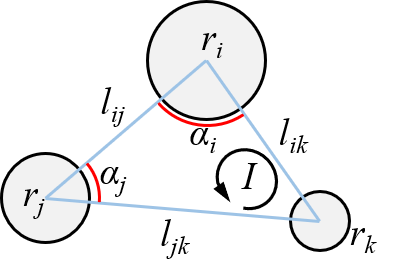
\includegraphics[width=0.3\textwidth]{Hanak三元组.png}
  \caption{Hanak描述子示意图}
  \label{fig:Hanak}
\end{figure}\par
需要事先保证按内角从大到小,排序为1、2和3,才能计算以下不变量,基于该计算结果,可求出当前不变量的不确定度,如下:
\begin{equation}
  \begin{aligned}
    u\left(\frac{2r_1}{l_1}\right)&=\frac{2}{l_1}\sqrt{u^2(r_1)+\left[\frac{r_1}{l_1}u(l_1)\right]^2}\\
    u\left(\frac{2r_2}{l_1}\right)&=\frac{2}{l_1}\sqrt{u^2(r_2)+\left[\frac{r_2}{l_1}u(l_1)\right]^2}\\
    u\left(\frac{2r_3}{l_1}\right)&=\frac{2}{l_1}\sqrt{u^2(r_3)+\left[\frac{r_3}{l_1}u(l_1)\right]^2}\\
    u(\cos\alpha_1)&=\frac{l_1}{l_2l_3}\sqrt{\cos^2\alpha_3u^2(l_2)+\cos^2\alpha_2u^2(l_3)+u^2(l_1)}\\
    u(\cos\alpha_2)&=\frac{l_2}{l_1l_3}\sqrt{\cos^2\alpha_3u^2(l_1)+\cos^2\alpha_1u^2(l_3)+u^2(l_2)}\\
    u(I_\mathrm{CW/CCW})&=0
  \end{aligned}
\end{equation}\par
其中,半径可近似认为由长短两轴平均而得:
\begin{equation*}
  r=\frac{a+b}{2}\implies u(r)=\frac{1}{2}\sqrt{u^2(a)+u^2(b)}
\end{equation*}\par
而最大边长$l_1$可由选定的两个顶点2和3计算所得,因此,其不确定度为:
\begin{equation*}
  u(l_1)=\frac{1}{l_1}\sqrt{(x_2-x_3)^2[u^2(x_2)+u^2(x_3)]+(y_2-y_3)^2[u^2(y_2)+u^2(y_3)]}
\end{equation*}\par
\subsection{Park描述子}
Hanak描述子仅是仿射不变量,因此不能用于着陆过程。Park\cite{parkRobustCraterTriangle2019}等人提出了利用交点计算的射影不变量,如图\ref{fig:Park}所示:
\begin{figure}[H]
  \centering
  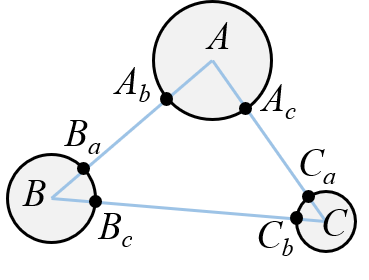
\includegraphics[width=0.3\textwidth]{Park三元组.png}
  \caption{Park描述子示意图}
  \label{fig:Park}
\end{figure}\par
其定义为利用六个交点计算的六组共30个不变量,按陨石坑的直径从大到小,分别为A、B和C,按照以下形式计算:
\begin{align*}
  I_{A_b}&=G(A_c,B_a,B_b,C_a,C_b)\\
  I_{A_c}&=G(A_b,B_a,B_c,C_a,C_b)\\
  I_{B_a}&=G(A_a,A_b,B_c,C_a,C_b)\\
  I_{B_c}&=G(A_a,A_c,B_a,C_a,C_b)\\
  I_{C_a}&=G(A_a,A_c,B_a,B_c,C_b)\\
  I_{C_b}&=G(A_a,A_c,B_a,B_c,C_a)\\
  G(x_1,x_2,x_3,x_4,x_5)&=\left[J(\mu),J(\nu),J\left(\frac{\mu}{\nu}\right),J\left(\frac{\nu-1}{\mu-1}\right),J\left(\frac{\mu(\nu-1)}{\nu(\mu-1)}\right)\right]\\
  \mu& = \frac{\triangle x_1x_2x_4\triangle x_1x_3x_5}{\triangle x_1x_3x_4\triangle x_1x_2x_5}\\
  \nu&=\frac{\triangle x_2x_1x_4\triangle x_2x_3x_5}{\triangle x_2x_3x_4\triangle x_2x_1x_5}\\
  J(x)&=\frac{2x^6-6x^5+9x^4-8x^3+9x^2-6x+2}{x^6-3x^5+3x^4-x^3+3x^2-3x+1}
\end{align*}\par
实验中表明,$J(x)$函数将全部不变量拉平了,并不利于描述,因此识别实验中取消$J(x)$部分,且$\mu$和$\nu$的数量级远远大于其他项,因此\textbr{只使用}$\mu$和$\nu$计算即可。关于从图像中确定交点,可利用特征值分解。可根据三个陨石坑中心点构造出三角形三边,以边$BC$和对应的两个顶点$B$和$C$为例:
\begin{equation*}
  \left\{
  \begin{aligned}
    \mathbf{x^\top Cx}&=0\\
    \mathbf{l^\top x}&=0  
  \end{aligned}
  \right.
\end{equation*}\par
因此,可根据高中所学知识,将直线方程写为$\mathbf{l}=[m,n,t]^\top$,代入至椭圆的一般式\ref{eq:ellipse}中,若设$n\neq 0$,可得:
\begin{equation}
  \left(A-2B\frac{m}{n}+C\frac{m^2}{n^2}\right)x^2+\left(-2B\frac{t}{n}+2C\frac{mt}{n^2}+2D-2E\frac{m}{n}\right)x+\left(C\frac{t^2}{n^2}-2E\frac{t}{n}+F\right)=0
  \label{eq:line}
\end{equation}\par
取定三个系数为:
\begin{align*}
  \left\{
    \begin{aligned}
      a &= A-2B\frac{m}{n}+C\frac{m^2}{n^2}\\
      b &= -2B\frac{t}{n}+2C\frac{mt}{n^2}+2D-2E\frac{m}{n}\\
      c &= C\frac{t^2}{n^2}-2E\frac{t}{n}+F
    \end{aligned}
  \right.
\end{align*}\par
使用二次方程求根公式即可得交点坐标的齐次表示为:
\begin{equation*}
  \mathbf{x}=\begin{bmatrix}
    x\\y\\1
  \end{bmatrix}=\begin{bmatrix}
    \frac{-b\pm\sqrt{b^2-4ac}}{2a}\\-\frac{m}{n}\left(\frac{-b\pm\sqrt{b^2-4ac}}{2a}\right)-\frac{t}{n}\\1
  \end{bmatrix}
\end{equation*}\par
当$n=0$时,以上公式失效,此时可将$x=\frac{t}{m}$代至椭圆一般式\ref{eq:ellipse}中,同理可得:
\begin{align*}
  \left\{
    \begin{aligned}
      a &= C\\
      b &= 2E-2B\frac{t}{m}\\
      c &= A\frac{t^2}{m^2}-2D\frac{t}{m}+F
    \end{aligned}
  \right.
\end{align*}\par
则交点坐标的齐次表示为:
\begin{equation*}
  \mathbf{x}=\begin{bmatrix}
    x\\y\\1
  \end{bmatrix}=\begin{bmatrix}
    -\frac{t}{m}\\\frac{-b\pm\sqrt{b^2-4ac}}{2a}\\1
  \end{bmatrix}
\end{equation*}\par
求解所得两个交点需要用对应位置的椭圆约束,以保证其在内侧,即向量$\overrightarrow{BB_c}$和$\overrightarrow{CB_c}$反向:
\begin{equation*}
  \overrightarrow{BB_c}\cdot\overrightarrow{CB_c}<0
\end{equation*}\par
由此可唯一确定六个交点,并解出共计30组不变量。由于该描述子实在是复杂到了一定的\textbr{境界},因此没有必要推导其不确定度了。
\subsection{互逆描述子}
互逆描述子由Quan\cite{quanInvariantsPairConics1992}等人提出,其定义为:
\begin{equation*}
  I_1 = \mathrm{tr}(\mathbf{C}_1^{-1}\mathbf{C}_2)\quad I_2 = \mathrm{tr}(\mathbf{C}_2^{-1}\mathbf{C}_1)
\end{equation*}\par
需要注意的是,\textbr{必须保证}$\det(\mathbf{C}_1)=\det(\mathbf{C}_2)=1$。为了计算该描述子的不确定度,首先将两个齐次矩阵定义为:
\begin{equation*}
  \mathbf{C}_1=\begin{bmatrix}
    A_1&B_1&D_1\\
    B_1&C_1&E_1\\
    D_1&E_1&F_1
  \end{bmatrix}\quad\mathbf{C}_2=\begin{bmatrix}
    A_2&B_2&D_2\\
    B_2&C_2&E_2\\
    D_2&E_2&F_2
  \end{bmatrix}
\end{equation*}\par
只计算$I_1$,根据矩阵求逆的定义,计算矩阵$\mathbf{C}_1$的伴随矩阵$\mathbf{C}_1^*$,并计算行列式:
\begin{equation*}
  \mathbf{C}_1^*=\begin{bmatrix}
   C_1F_1-E_1^2 & D_1E_1-B_1F_1 & B_1E_1-C_1D_1\\
    D_1E_1-B_1F_1 & A_1F_1-D_1^2 & B_1D_1-A_1E_1\\
    B_1E_1-C_1D_1 & B_1D_1-A_1E_1 & A_1C_1-B_1^2
  \end{bmatrix}\quad\det(\mathbf{C}_1)=A_1C_1F_1+2B_1D_1E_1-A_1E_1^2-C_1D_1^2-B_1^2F_1
\end{equation*}\par
然后,只需要计算$\mathbf{C}_1^{-1}\mathbf{C}_2$的主对角线元素之和即可:
\begin{align*}
 ( \mathbf{C}_1^{-1}\mathbf{C}_2)_{11}&= \frac{1}{\det(\mathbf{C}_1)}\left[(C_1F_1-E_1^2)A_2+(D_1E_1-B_1F_1)B_2+(B_1E_1-C_1D_1)D_2\right]\\
  ( \mathbf{C}_1^{-1}\mathbf{C}_2)_{22}&= \frac{1}{\det(\mathbf{C}_1)}\left[(D_1E_1-B_1F_1)B_2+(A_1F_1-D_1^2)C_2+(B_1D_1-A_1E_1)E_2\right]\\
  ( \mathbf{C}_1^{-1}\mathbf{C}_2)_{33}&= \frac{1}{\det(\mathbf{C}_1)}\left[(B_1E_1-C_1D_1)D_2+(B_1D_1-A_1E_1)E_2+(A_1C_1-B_1^2)F_2\right]
\end{align*}\par
因此,$I_1$的闭式解为:
\begin{align*}
  I_1&=\frac{1}{\det(\mathbf{C}_1)}\left[(C_1F_1-E_1^2)A_2+2(D_1E_1-B_1F_1)B_2+2(B_1E_1-C_1D_1)D_2\right.\\
  &\left.+(A_1F_1-D_1^2)C_2+2(B_1D_1-A_1E_1)E_2+(A_1C_1-B_1^2)F_2\right]
\end{align*}\par
为了求解该描述子的不确定度,首先计算$\det(\mathbf{C}_1)$对六个元素分量的偏导数,有:
\begin{align*}
  \pdiff{\det(\mathbf{C}_1)}{A_1}&=C_1F_1-E_1^2\\
  \pdiff{\det(\mathbf{C}_1)}{B_1}&=2D_1E_1-2B_1F_1\\
  \pdiff{\det(\mathbf{C}_1)}{C_1}&=A_1F_1-D_1^2\\
  \pdiff{\det(\mathbf{C}_1)}{D_1}&=2B_1E_1-2C_1D_1\\
  \pdiff{\det(\mathbf{C}_1)}{E_1}&=2B_1D_1-2A_1E_1
\end{align*}
\begin{equation*}
  \pdiff{\det(\mathbf{C}_1)}{F_1}=A_1C_1-B_1^2
\end{equation*}\par
然后,计算分子部分$N_1$对十二个元素的各个偏导数,有:
\begin{align*}
  \pdiff{N_1}{A_1}&=F_1C_2+C_1F_2-2E_1E_2\\
  \pdiff{N_1}{B_1}&=2E_1D_2+2D_1E_2-2F_1B_2-2B_1F_2\\
  \pdiff{N_1}{C_1}&=F_1A_2+A_1F_2-2D_1D_2\\
  \pdiff{N_1}{D_1}&=2E_1B_2+2B_1E_2-2C_1D_2-2D_1C_2\\
  \pdiff{N_1}{E_1}&=2D_1B_2+2B_1D_2-2A_1E_2-2E_1A_2\\
  \pdiff{N_1}{F_1}&=A_1C_2+C_1A_2-2B_1B_2\\
  \pdiff{N_1}{A_2}&=C_1F_1-E_1^2\\
  \pdiff{N_1}{B_2}&=2D_1E_1-2B_1F_1\\
  \pdiff{N_1}{C_2}&=A_1F_1-D_1^2\\
  \pdiff{N_1}{D_2}&=2B_1E_1-2C_1D_1\\
  \pdiff{N_1}{E_2}&=2B_1D_1-2A_1E_1\\
  \pdiff{N_1}{F_2}&=A_1C_1-B_1^2
\end{align*}\par
代入后可取得$u(I_1)$的表达式。
\subsection{距离描述子}
实践中,发现互逆描述子需要保持行列式归一,引入了额外的计算量,当椭圆被压扁时,行列式接近于0,因此增加了数值不稳定。本人提出了具有以下形式的距离描述子:
\begin{equation*}
  I_1 = \frac{\mathbf{x}_2^\top\mathbf{C}_1\mathbf{x}_2}{\mathbf{x}_1^\top\mathbf{C}_1\mathbf{x}_1}=\frac{N_1}{D_1}\quad I_2 = \frac{\mathbf{x}_1^\top\mathbf{C}_2\mathbf{x}_1}{\mathbf{x}_2^\top\mathbf{C}_2\mathbf{x}_2}=\frac{N_2}{D_2}
\end{equation*}\par
其形式尚未见于任何文献报道,经过实验发现,其分布比互逆描述子更均匀,且不需要计算两个椭圆的行列式。式中的$\mathbf{x}_1$和$\mathbf{x}_2$是以齐次坐标表示的两个椭圆中心点。其几何意义为:两个圆中心距离与圆各自半径之比,是平面下的射影不变量。不确定度服从以下形式:
\begin{equation*}
  u(I_1)=
\end{equation*}
同理,可以推导该描述子的不确定度,借助椭圆中心点的不确定度公式\ref{eq:center-uncertainty},可得:
\begin{align*}
  \left\{\begin{aligned}
    \pdiff{N_1}{A_1}&=x_{01}^2\\
    \pdiff{N_1}{B_1}&=2x_{01}y_{01}\\
    \pdiff{N_1}{C_1}&=y_{01}^2\\
    \pdiff{N_1}{D_1}&=2x_{01}\\
    \pdiff{N_1}{E_1}&=2y_{01}\\
    \pdiff{N_1}{F_1}&=1
  \end{aligned}\right.\quad\left\{\begin{aligned}
    \pdiff{N_1}{A_2}&=2\pdiff{\mathbf{x}_2^\top}{A_2}\mathbf{C}_1\mathbf{x}_2\\
    \pdiff{N_1}{B_2}&=2\pdiff{\mathbf{x}_2^\top}{B_2}\mathbf{C}_1\mathbf{x}_2\\
    \pdiff{N_1}{C_2}&=2\pdiff{\mathbf{x}_2^\top}{C_2}\mathbf{C}_1\mathbf{x}_2\\
    \pdiff{N_1}{D_2}&=2\pdiff{\mathbf{x}_2^\top}{D_2}\mathbf{C}_1\mathbf{x}_2\\
    \pdiff{N_1}{E_2}&=2\pdiff{\mathbf{x}_2^\top}{E_2}\mathbf{C}_1\mathbf{x}_2\\
    \pdiff{N_1}{F_2}&=2\pdiff{\mathbf{x}_2^\top}{F_2}\mathbf{C}_1\mathbf{x}_2
  \end{aligned}\right.\quad\quad\quad \left\{\begin{aligned}
    \pdiff{N_2}{A_2}&=x_{02}^2\\
    \pdiff{N_2}{B_2}&=2x_{02}y_{02}\\
    \pdiff{N_2}{C_2}&=y_{02}^2\\
    \pdiff{N_2}{D_2}&=2x_{02}\\
    \pdiff{N_2}{E_2}&=2y_{02}\\
    \pdiff{N_2}{F_2}&=1
  \end{aligned}\right.\quad \left\{\begin{aligned}
    \pdiff{N_2}{A_1}&=2\pdiff{\mathbf{x}_1^\top}{A_1}\mathbf{C}_2\mathbf{x}_1\\
    \pdiff{N_2}{B_1}&=2\pdiff{\mathbf{x}_1^\top}{B_1}\mathbf{C}_2\mathbf{x_1}\\
    \pdiff{N_2}{C_1}&=2\pdiff{\mathbf{x}_1^\top}{C_1}\mathbf{C}_2\mathbf{x_1}\\
    \pdiff{N_2}{D_1}&=2\pdiff{\mathbf{x}_1^\top}{D_1}\mathbf{C}_2\mathbf{x_1}\\
    \pdiff{N_2}{E_1}&=2\pdiff{\mathbf{x}_1^\top}{E_1}\mathbf{C}_2\mathbf{x_1}\\
    \pdiff{N_2}{F_1}&=2\pdiff{\mathbf{x}_1^\top}{F_1}\mathbf{C}_2\mathbf{x_1}
  \end{aligned}\right.
\end{align*}\par
同理,可以计算分母部分的偏导数:
\begin{align*}
  \left\{\begin{aligned}
    \pdiff{D_1}{A_1}&=x_{01}^2+2\pdiff{\mathbf{x}_1^\top}{A_1}\mathbf{C}_1\mathbf{x}_1\\
    \pdiff{D_1}{B_1}&=2x_{01}y_{01}+2\pdiff{\mathbf{x}_1^\top}{B_1}\mathbf{C}_1\mathbf{x}_1\\
    \pdiff{D_1}{C_1}&=y_{01}^2+2\pdiff{\mathbf{x}_1^\top}{C_1}\mathbf{C}_1\mathbf{x}_1\\
    \pdiff{D_1}{D_1}&=2x_{01}+2\pdiff{\mathbf{x}_1^\top}{D_1}\mathbf{C}_1\mathbf{x}_1\\
    \pdiff{D_1}{E_1}&=2y_{01}+2\pdiff{\mathbf{x}_1^\top}{E_1}\mathbf{C}_1\mathbf{x}_1\\
    \pdiff{D_1}{F_1}&=1+2\pdiff{\mathbf{x}_1^\top}{F_1}\mathbf{C}_1\mathbf{x}_1
  \end{aligned}\right.\quad \left\{\begin{aligned}
    \pdiff{D_1}{A_2}&=x_{02}^2+2\pdiff{\mathbf{x}_2^\top}{A_2}\mathbf{C}_2\mathbf{x}_2\\
    \pdiff{D_1}{B_2}&=2x_{02}y_{02}+2\pdiff{\mathbf{x}_2^\top}{B_2}\mathbf{C}_2\mathbf{x}_2\\
    \pdiff{D_1}{C_2}&=y_{02}^2+2\pdiff{\mathbf{x}_2^\top}{C_2}\mathbf{C}_2\mathbf{x}_2\\
    \pdiff{D_1}{D_2}&=2x_{02}+2\pdiff{\mathbf{x}_2^\top}{D_2}\mathbf{C}_2\mathbf{x}_2\\
    \pdiff{D_1}{E_2}&=2y_{02}+2\pdiff{\mathbf{x}_2^\top}{E_2}\mathbf{C}_2\mathbf{x}_2\\
    \pdiff{D_1}{F_2}&=1+2\pdiff{\mathbf{x}_2^\top}{F_2}\mathbf{C}_2\mathbf{x}_2
  \end{aligned}\right.
\end{align*}\par
形式非常美观,可以直接代入公式\ref{eq:center-uncertainty}直接计算不确定度。
\newpage
\printbibliography[heading=bibliography,title=参考文献]
\end{document}
